% mn2esample.tex
%
% v2.1 released 22nd May 2002 (G. Hutton)
%
% The mnsample.tex file has been amended to highlight
% the proper use of LaTeX2e code with the class file
% and using natbib cross-referencing. These changes
% do not reflect the original paper by A. V. Raveendran.
%
% Previous versions of this sample document were
% compatible with the LaTeX 2.09 style file mn.sty
% v1.2 released 5th September 1994 (M. Reed)
% v1.1 released 18th July 1994
% v1.0 released 28th January 1994

\documentclass[useAMS,usenatbib]{mn2e}
\usepackage{graphicx}
\usepackage{amsmath}


% If your system does not have the AMS fonts version 2.0 installed, then
% remove the useAMS option.
%
% useAMS allows you to obtain upright Greek characters.
% e.g. \umu, \upi etc.  See the section on "Upright Greek characters" in
% this guide for further information.
%
% If you are using AMS 2.0 fonts, bold math letters/symbols are available
% at a larger range of sizes for NFSS release 1 and 2 (using \boldmath or
% preferably \bmath).
%
% The usenatbib command allows the use of Patrick Daly's natbib.sty for
% cross-referencing.
%
% If you wish to typeset the paper in Times font (if you do not have the
% PostScript Type 1 Computer Modern fonts you will need to do this to get
% smoother fonts in a PDF file) then uncomment the next line
% \usepackage{Times}

%%%%% AUTHORS - PLACE YOUR OWN MACROS HERE %%%%%

\title[Results of two stellar occultations by Ceres]{Results of two stellar occultations by dwarf planet (1) Ceres}
\author[A. V. Raveendran and A. N. Other]{A. V. Raveendran$^{1}$\thanks{E-mail:
email@address (AVR); otheremail@otheraddress (ANO)} and A. N.
Other$^{2}$\footnotemark[1]\thanks{}\\
$^{1}$Observat\'orio do Valongo/UFRJ, Ladeira Pedro Ant\^onio 43,
CEP 20.080-090 Rio de Janeiro - RJ, Brazil\\
$^{2}$Observat\'orio Nacional/MCT, R. General Jos\'e Cristino 77,
CEP 20921-400 Rio de Janeiro - RJ, Brazil}
\begin{document}

\date{Accepted . Received ; in original form }

\pagerange{\pageref{firstpage}--\pageref{lastpage}} \pubyear{2015}

\maketitle

\label{firstpage}

\begin{abstract}
Abstract
\end{abstract}

\begin{keywords}
minor planets, asteroids: individual (1, Ceres) - occultations - planets and satellites: fundamental parameters
\end{keywords}

\section{Introduction}

Ceres is the sole exemplar of a dwarf planet in the inner Solar System. Far from being a mere taxonomic information, this suggests the great impact its study can have on the understanding of planetary formation and evolution of the Solar System. Indeed, it was proposed that Ceres could have its origin as a transneptunian object, later scattered to the Main Belt due to the giant planets' migration predicted by the `Nice Model'. It may well had been formed close to its current location, however, even on this scenario, the dynamical history of the Solar System must have let its signatures on Ceres. Not only on the late heavy bombardment features that might exist on its surface, but also on its volatiles, which could have been transported from the outer region.

Since the 1970's it has been speculated that Ceres could contain water ice, what was recently verified \citep{Kuppers2014}. Although the water regime on this object is still unknown, some internal structure models suggest the existence of a water ice -- or even a liquid water -- layer. Yet the very question of whether Ceres suffered differentiation is open and, on the assumption of an affirmative answer, it is natural to ask if it ever had tectonics, how its geological evolution was, and if it is still active. Inarguably NASA's \textit{Dawn} mission will shed light on several open issues concerning Ceres.

Owning approximately one fifth of the whole Main Belt's mass, Ceres is expected to have an equilibrium figure, i.e. a Maclaurin or a Jacobi ellipsoid. In fact, direct observations of Ceres by means of adaptive optics confirmed it to be an oblate spheroid \citep{Drummond2014}. The precise knowledge of its shape and dimensions is important, for the models of density, internal structure and differentiation can depend on the size and oblateness of the body.

The best ground-based technique for determining shape and size of a faraway object is the study of its shadow, cast by a star during an occultation. Since the 1960's occultations have provided measurements of hundreds of asteroids, thanks partially to the proficuous professional-amateur collaboration on the field. More recently, this technique has been applied to objects of the outer Solar System and has unveiled outstanding features of distant bodies, e.g. the ring system around the Centaur (10199) Chariklo \citep{BragaRibas2014}.

The first stellar occultation by Ceres was observed in 1984 \citep{Millis1987} and led to the determination of its size to the precision of the kilometre, in a time when the uncertainties were often ten times larger. The low apparent magnitude of Ceres, if compared to most asteroids, imposes a somewhat strong constraint on the stars capable of causing a detectable magnitude drop when occulted. For instance, after the 1984 event, to our knowledge, only four like this have been observed. Two of them had only two chords each, not sufficient, thus, for providing accurate results\footnote{These events took place on 22 August 1994 and 30 October 2010.}. The two remaining events, which occurred on 17 August 2010 and 25 October 2013, are reported on the present work. The former was observed in Brazil from 4 stations, while the latter was from the United States and led to 9 chords. Throughout the paper we shall refer to these events as the `2010' and the `2013 occultation'.

Both events were foreseen by Steve Preston\footnote{Predictions are published at http://asteroidoccultation.com.} on behalf of the International Occultation Timing Association, during routine prediction of asteroidal occultations of bright stars.

This work is organized as follows. In Sections 2 and 3 we analyse, on this order, the 2010 and the 2013 events. The comparison of both results to those on the literature is carried out in Section 4.






\section[]{The 2010 occultation}

\subsection{Observations}

%Asteroidal occultations of bright stars are routinely predicted by Steve Preston\footnote{Predictions are published at http://asteroidoccultation.com.}, on behalf of the International Occultation Timing Association. Within this context it was identified that on 17 August 2010 Ceres would occult the star TYC 6833-163-1 (UCAC2 20678706), which has magnitude $\text{K}=9.18$ and whose ICRF/J200 position is \citep{Zacharias2004}:
%
On 17 August 2010 Ceres was predicted to occult the star TYC 6833-163-1 (UCAC2 20678706), which has magnitude $K=9.18$ and whose ICRF/J200 position is \citep{Zacharias2004}:
%
\begin{equation}
\left\{ 
  \begin{array}{l l}
    \alpha = 17^{\text{h}}18^{\text{m}}29^{\text{s}}.008\\
    \delta = -27\degr 26\arcmin 38\arcsec.890.
  \end{array}
\right.
\end{equation}
%
The shadow's path would cross South America, the Atlantic and reach the south part of Africa.

\begin{figure}
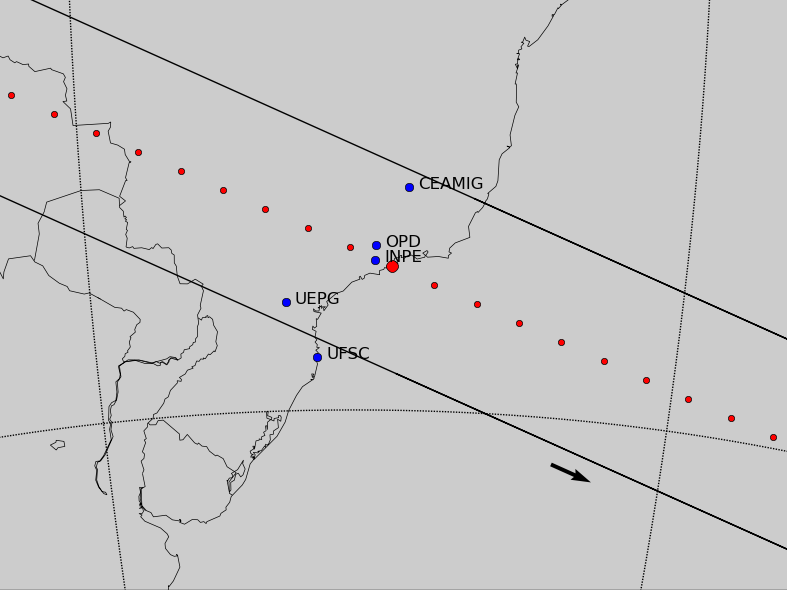
\includegraphics[scale=0.42]{figures/Ceres_2010.png} 
\caption{Post-occultation reconstruction of Ceres' shadow path on Earth for the 2010 August 17 event. The big red dot is the geocentric closest approach at 22:40:25 UT. The small red ones represent the centre of the shadow separated by one minute, shadow moves from the left to the right. Blue dots are the sites that have observed the event. As described in text, UFSC had a negative chord.
\label{Fig: Ceres-2010-map}}
\end{figure}

Observations were carried out in Brazil at five stations as displayed in Table~1 and Fig.~\ref{Fig: Ceres-2010-map}. The occultation was detected on four of them. Among these, one started the shots with the event already in progress and only provided star's reappearance time; the other three recorded the whole phenomenon.

A remarkable circumstance of this event was the low velocity of Ceres: only 3.9 km s$^{-1}$ in the plane of the sky. Therefore, even exposures of a few seconds would translate in a relevant spatial resolution.


[Falar sobre a quest\~ao do tempo em cada corda. A leitura do header era no segundo inteiro? Foi analisada a cad\^encia das imagens? Qual a precis\~ao?]

[Durante o per\'iodo de observac\~ao Ceres rodou apenas 3.1$\degr$. Mas isso n\~ao \'e relevante no caso de Maclaurin...]

\begin{table*}
 \centering
 \begin{minipage}{140mm}
  \caption{Circumstances of observation for all observing stations of the 2010 event. \label{Tab: obs-2010}}
  \begin{tabular}{@{}lccccc}
  \hline
     Site & Longitude & Telescope & Exposure & Result & Observer  \\
          & Latitude  & Aperture  & Cycle time & Ingress & \\          
          & Height    & Camera    &    S/N    & Egress    & \\          
\hline
 Belo Horizonte & 43$\degr$59'51.1'' W & LX200 & 5 s & Positive & C. Jacques  \\
 CEAMIG-REA &19$\degr$49'49.0'' S & 31 cm & 12 s & 22:39:03.9 $\pm$ 0.6 &  E. Pimentel \\
            & 825 m                &       &     & 22:40:20 $\pm$ 5 &   \\
 & & & & & \\
 Pico dos Dias    & 45$\degr$34'45.1'' W &       & 1 s & Positive & J. I. B. Camargo \\
 OPD/LNA    &22$\degr$32'03.7'' S & 60 cm & 2 s & 22:37:30.3 $\pm$ 0.6 &  G. B. Rossi \\
            & 1864 m               &       &     & 22:41:55.3 $\pm$ 0.7 &              \\
 & & & & & \\
 S\~ao Jos\'e dos       & 45$\degr$51'44.0'' W &  C11  & 2 s & Egress only & A. C. Milone\\
 Campos       &23$\degr$12'33.0'' S & 28 cm & 5 s & Start: 22:39:44 & T. Maldonado\\
 INPE      & 975 m                & SBIG ST7 &     & 22:42:03.0 $\pm$ 0.2 & M. Okada    \\
 & & & & & \\
 Ponta Grossa       & 50$\degr$05'56.0'' W & RCX 400 &30 s & Positive & M. Emilio   \\
 UEPG       &25$\degr$05'22.2'' S & 40 cm & 52 s & 22:37:17 $\pm$ 13 & L. Mehret   \\
            & 910 m                & SBIG STL6E &     & 22:39:56 $\pm$ 13 & \\
 & & & & & \\
 Florian\'opolis       & 48$\degr$31'20.5'' W &       & 3 s & No occultation  & W. Schoenell\\
 UFSC       &27$\degr$36'12.3'' S & 28 cm & 6 s&  & A. J. T. Mello\\
            & 20 m                 &       &  &         & F. R. Herpich \\
\hline
\end{tabular}
\end{minipage}
\end{table*}




\subsection{Light curves and timing \label{Sec: light-curve-2010}}

The flux of the star in the five occultation chords was obtained from the FITS images with the Platform for Reduction of Astronomical Images Automatically (PRAIA) \citep{2011gfun.conf...85A}. The light curves were normalized to an unocculted star flux. Additionally --with exception of INPE-- they were were normalized by fitting a polynomial curve (of first or second order) outside the flux drop, so that the flux ratio was set to 1 outside the occultation.

The start and end times of the occultation were obtained for each light curve by fitting a sharp edge occultation model. This model is convolved by Fresnel diffraction, the CCD bandwidth, the stellar aparent diameter, and the finite integration time; see \cite{Widemann2009}.

The Fresnel scale ($F = \sqrt{\lambda D/2}$) for the present Ceres' geocentric distance $D = 2.29 \text{ au} = 3.42 \times 10^{8}$~km is 0.3~km for a typical wavelength of $\lambda = 0.65$~$\micron$. The star diameter is estimated using the formulae of \cite{vanBelle1999}. Its $B$, $V$, and $K$ apparent magnitudes are 12.00, 11.78 and 9.18, respectively, in the Tycho catalog \citep{Hog2000}. This yields a diameter of about 0.11~km projected at Ceres' distance. The smallest integration time used in the positive observations was 1.0~s, which translates to almost 3.9~km in the celestial plane. Therefore, the occultation light curves are largely dominated by the integration times, not by Fresnel diffraction or star diameter.

The occultation fits consist in minimizing a classical $\chi^{2}$ function for each light curve, as described in \cite{Sicardy2011}. The free parameter to adjust is the ingress (disappearance) or egress (reappearance) time $t_{occ}$, which provides the minimum value of $\chi^{2}$, denoted as $\chi^{2}_{min}$. The best fittings to the occultation light curves are shown in Fig.~\ref{Fig: Ceres-2010-curves}, and the derived occultation times are listed in Table~\ref{Tab: obs-2010}.


\begin{figure}
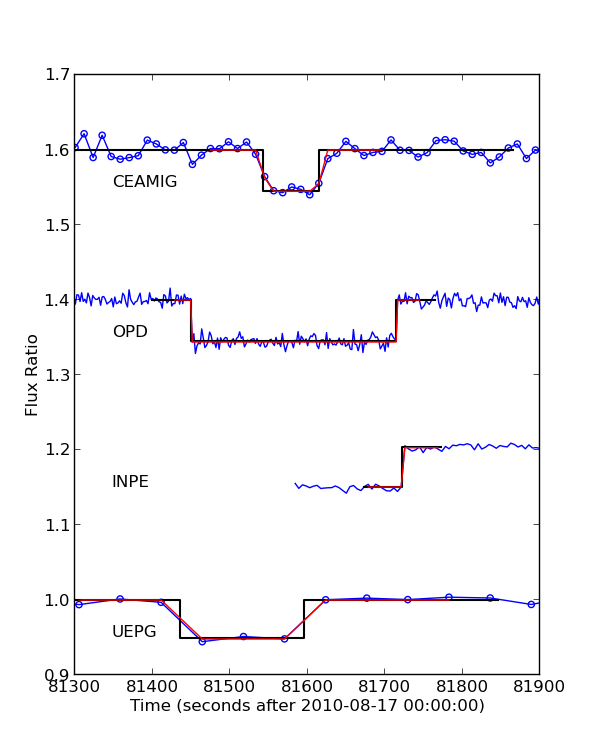
\includegraphics[scale=0.58]{figures/Ceres_2010_fluxratio.png} 
\caption{The four occultation light curves normalized and vertically shifted by a factor of 0.2 for better viewing. The solid black lines are the best fit of the square-well model to the data. Red lines are the square-well model convoluted with the Fresnel diffraction, the star diameter, and the applied exposure time. The mid-times of the occultations do not coincide due to the propagation delays of the shadow due to the distinct longitude of the sites. Exposures at INPE started after the immersion, as explained in the text. \label{Fig: Ceres-2010-curves}}
\end{figure}


\subsection{Limb fitting methodology} \label{Sec: limbfittingmethod}

The methodology used to analyse Ceres' profile from the observations is the same described by \cite{Sicardy2011} and \cite{BragaRibas2013}. To each combination of site position and recorded ingress/egress time, together with star coordinates and Ceres' ephemeris, corresponds a point $(f_{i,obs},g_{i,obs})$ on the plane of the sky. The collection of those points ideally determines the apparent limb of Ceres.

We adopt an elliptic model for the limb profile, resulting from the projection of an oblate spheroid onto the sky plane. This model is supported by the work of \cite{Drummond2014}, by means of direct imaging of Ceres. Hence, we have $N=7$ chord extremities to adjust the $M=5$ parameters which define an ellipse: apparent semimajor and semiminor axis --$a^\prime$ and $b^\prime$, respectively--, position angle $P$ of its semiminor axis and the position $(f_c,g_c)$ of its centre with respect to the occulted star\footnote{The coordinates $f_{c}$ and $g_{c}$, in kilometres, are calculated using the JPL\#33 Ceres' ephemeris and the occulted star's position. They are positive toward the local celestial east and north, respectively. The position angle $P$ is counted positively from the direction of local celestial north to celestial east.}. The apparent oblateness can be defined by $\epsilon^\prime = 1 - (b^\prime/a^\prime)$. We define the number of degrees of freedom of the problem as $\mathcal{N} \equiv N - M$.

%We adopt an elliptic model for the limb profile, resulting from the projection of an oblate spheroid onto the sky plane. This model is supported by the work of \cite{Drummond2014}, by means of direct imaging of Ceres. Hence, we have $N=7$ chord extremities to adjust the $M=5$ parameters which define an ellipse: apparent semimajor and semiminor axis -- $a^\prime$ and $b^\prime$, respectively --, position angle $P$ of its semiminor axis and the position $(f_c,g_c)$ of its centre with respect to the occulted star\footnote{The coordinates $f_{c}$ and $g_{c}$, in kilometres, are calculated using the JPL\#33 Ceres' ephemeris and the occulted star's position. They are positive toward the local celestial east and north, respectively. The position angle $P$ is counted positively from the direction of local celestial north to celestial east.}. The first two parameters can be interchanged with the oblateness and the equivalent radius, defined, on this order, by $\epsilon^\prime = 1 - (b^\prime/a^\prime)$ and $R_{equiv} \equiv \sqrt{a^\prime b^\prime} = a^\prime\sqrt{1-\epsilon^\prime}$. We define the number of degrees of freedom of the problem as $\mathcal{N} \equiv N - M$.

The apparent oblateness is related to the true one $\epsilon$ through
%
\begin{equation}
\epsilon^\prime = 1 - \sqrt{\cos^2(\zeta) + (1-\epsilon)^2\sin^2(\zeta)},
\label{TrueObla}
\end{equation}
%
where $\zeta$ is the polar aspect angle, encompassed by the (true) polar semiminor axis and the line of sight. Of course, the apparent semimajor axis $a^\prime$ equals the equatorial radius $R_{equa}$ of the ellipsoid.

%Correspondence between true and apparent figures depends on the polar aspect angle $\zeta$, encompassed by the (true) polar $b$-axis and the line of sight. The apparent oblateness is related to the true one, $\epsilon$, through

The search for the best-fitting ellipse is carried out by minimizing the reduced $\chi^2$ function:
%
\begin{equation}
\chi^2_r = \frac{1}{\mathcal{N}} \sum_{i=1}^N \frac{1}{\sigma_i^2}  \left[ (f_{i,obs}-f_{i,cal})^2 + (g_{i,obs}-g_{i,cal})^2\right].
\end{equation}
%
Here $\sigma_i$ is the radial uncertainty of the $i$th chord extremity, obtained by multiplying the time uncertainty reported in Table~1 by the normal velocity of the star (with respect to the limb model). $f_{i,cal}$ and $g_{i,cal}$ are the coordinates of the point on the model ellipse, where a line that goes from the centre of the model to the data point $(f_{i,obs},g_{i,obs})$ intersects the ellipse.%:
%
%\begin{equation}
%f_{i,cal} \equiv f_{i,obs} + \rho \cos(\theta), \quad g_{i,cal} \equiv %g_{i,obs} + \rho \sin(\theta),
%\end{equation}
%
%with:
%\begin{equation}
%\theta \equiv \arctan\left( \frac{g_{i,obs}-g_{c}}{f_{i,obs}-f_{c}} %\right) ,
%\end{equation}
%
%\begin{equation}
%\rho \equiv a^\prime b^\prime / \sqrt{[a^\prime\sin(\theta+P)]^2 +[b^\prime\cos(\theta+P)]^2 }.
%\end{equation}

Evaluation of the reduced $\chi^2$ function over the $\lbrace R_{equa}, \epsilon^\prime, P, f_c, g_c \rbrace$--space produces a map related to the likelihood of a solution. For instance, the 1--sigma reported time uncertainties correspond to the subset of the parameter space for which $\chi^2_r$ lies between ${\chi^2_r}_{min}$ and ${\chi^2_r}_{min} + 1$. This allows the determination of the error bars of the physical parameters. It is worthwhile to mention that we consider all the uncertainty as due to timing issues.





\subsection{Limb fitting solutions}\label{Sec: limbfitting-2010}

Two possible solutions were considered for the limb fitting. The first is the nominal one, which consists of determining the five parameters that characterize an ellipse from the seven observed contacts. As we shortly show, it led to a rather large error bar on the position angle. Furthermore, the nominal solution solely is not capable of returning the true oblateness, which can be evaluated through equation \eqref{TrueObla}, provided that the angle $\zeta$ is known.% or constrained by some physical hypothesis.

From observations by adaptive optics spanning a 10-year period, \cite{Drummond2014} determined the position of Ceres' polar axis within a range of only 3$\degr$:
\begin{equation}
%\left\{ 
%\begin{array}{l}
\alpha = (287 \pm 3) \degr, \quad %\\
\delta = (+64 \pm 3) \degr,
%\end{array} \right .
\label{Pole}
\end{equation}
%
in equatorial J2000 coordinates. Together with Ceres' ephemeris at the moment of the occultation, this corresponds to the polar aspect angle $\zeta = 86.1\degr$, which is very close to an equator-on geometry. Hence, we expect true figures to be similar to apparent ones.

The knowledge of Ceres' pole not only allows the determination of its polar aspect, it suffices to set its position angle. Therefore \eqref{Pole} may act as a constraint for $P$, and a second solution can be obtained by probing the parameter space with the restriction that the position angle is confined to the range that follows from \eqref{Pole}. We call this the ``pole-constrained solution''.


\subsubsection{Nominal solution}

With the seven observed contacts it is possible to adjust the five parameters which define an ellipse. For the best-fitting solution we find $\chi^2_{r,min} = 0.24$, which could be interpreted as a slightly overestimation of the error bars with regard to the good quality of the fit. However, inasmuch as the problem has only two degrees of freedom, it is far from the statistical realm and low $\chi^2_{r,min}$ may eventually happen.

The resulting values of equatorial diameter, oblateness, position angle and centre coordinates are presented in the second column of Table~2.%, and the corresponding ellipse is plotted with the observed chords in Fig.~2.
% The equivalent radius of the best-fitting solution is $R_{equiv} = 469 \pm 10$ km.

Already mentioned, the parameter with the largest uncertainty is the position angle: spanning on a 20$\degr$ interval, its determination has a relative precision worse than 10$\%$. Clearly, the coordinates of Ceres' pole (\ref{Pole}) can impose a strong constraint on the position angle, as the next solution shows.

Finally, the correction to the oblateness due to Ceres' polar aspect angle lies within the 1-sigma error bar and has no statistical relevance; hence $\epsilon = 0.08 \pm 0.03$.





\subsubsection{Pole-constrained solution}

At the moment of the occultation, the coordinates (\ref{Pole}) of Ceres' rotational pole correspond to the position angle $P = (12 \pm 3)\degr$. Exploration of the parameter space, restricted to ellipses whose position angle lie on this range, results in the pole-constrained solution. The related physical parameters are displayed on the third column of Table~2, while the best-fitting solution is depicted in Fig.\ref{Fig:Ceres-2010-body}.

We notice that the constraint corresponds to the upper limit of nominal solution's 1-sigma error bar for $P$. On the other hand, it selects the smallest values of equatorial radius, improving its determination by a factor of about 2. Notwithstanding, oblateness' figures remain the same.


\begin{table*}
 \centering
 \begin{minipage}{140mm}
  \caption{Results of limb fitting to the data of the 2010 and 2013 events.}
  \begin{tabular}{@{}lcccc}
  \hline
     Solution & 2010/Nominal & 2010/Pole-constrained & 2013/Nominal & 2013/Pole-constrained \\
\hline
Equatorial diameter (km) & 982 $\pm$ 14 & 972 $\pm$ 6  & 971 $\pm$ 7  & 971 $\pm$ 7\\
%Equatorial diameter (km) & 491 $\pm$ 7  & 486 $\pm$ 3  & 485.5 $\pm$ 3.5 & 485.5 $\pm$ 3.5\\
True oblateness        & 0.08 $\pm$ 0.03 & 0.08 $\pm$ 0.03 & 0.08 $\pm$ 0.04 & 0.08 $\pm$ 0.04\\
Position angle (deg)   & 5 $\pm$ 10    & 12 $\pm$ 3 (*)& 22 $\pm$ 5    & 25 $\pm$ 3 (*)\\
$f_c$ (km)             & 133 $\pm$ 9   & 138 $\pm$ 5   & 77 $\pm$ 6    & 78 $\pm$ 6\\
$g_c$ (km)             & -17 $\pm$ 15  & -11 $\pm$ 11  & 13 $\pm$ 16   & 13 $\pm$ 16\\
$\chi^2_{r,min}$       & 0.24          &  0.42         & 1.27          & 1.27\\
\hline
\end{tabular}
\textbf{Notes.} Error bars are at 1-sigma level.
(*) Position angle derived from Ceres' rotational pole coordinates determined by \cite{Drummond2014}.
\end{minipage}
\end{table*}

\begin{figure}
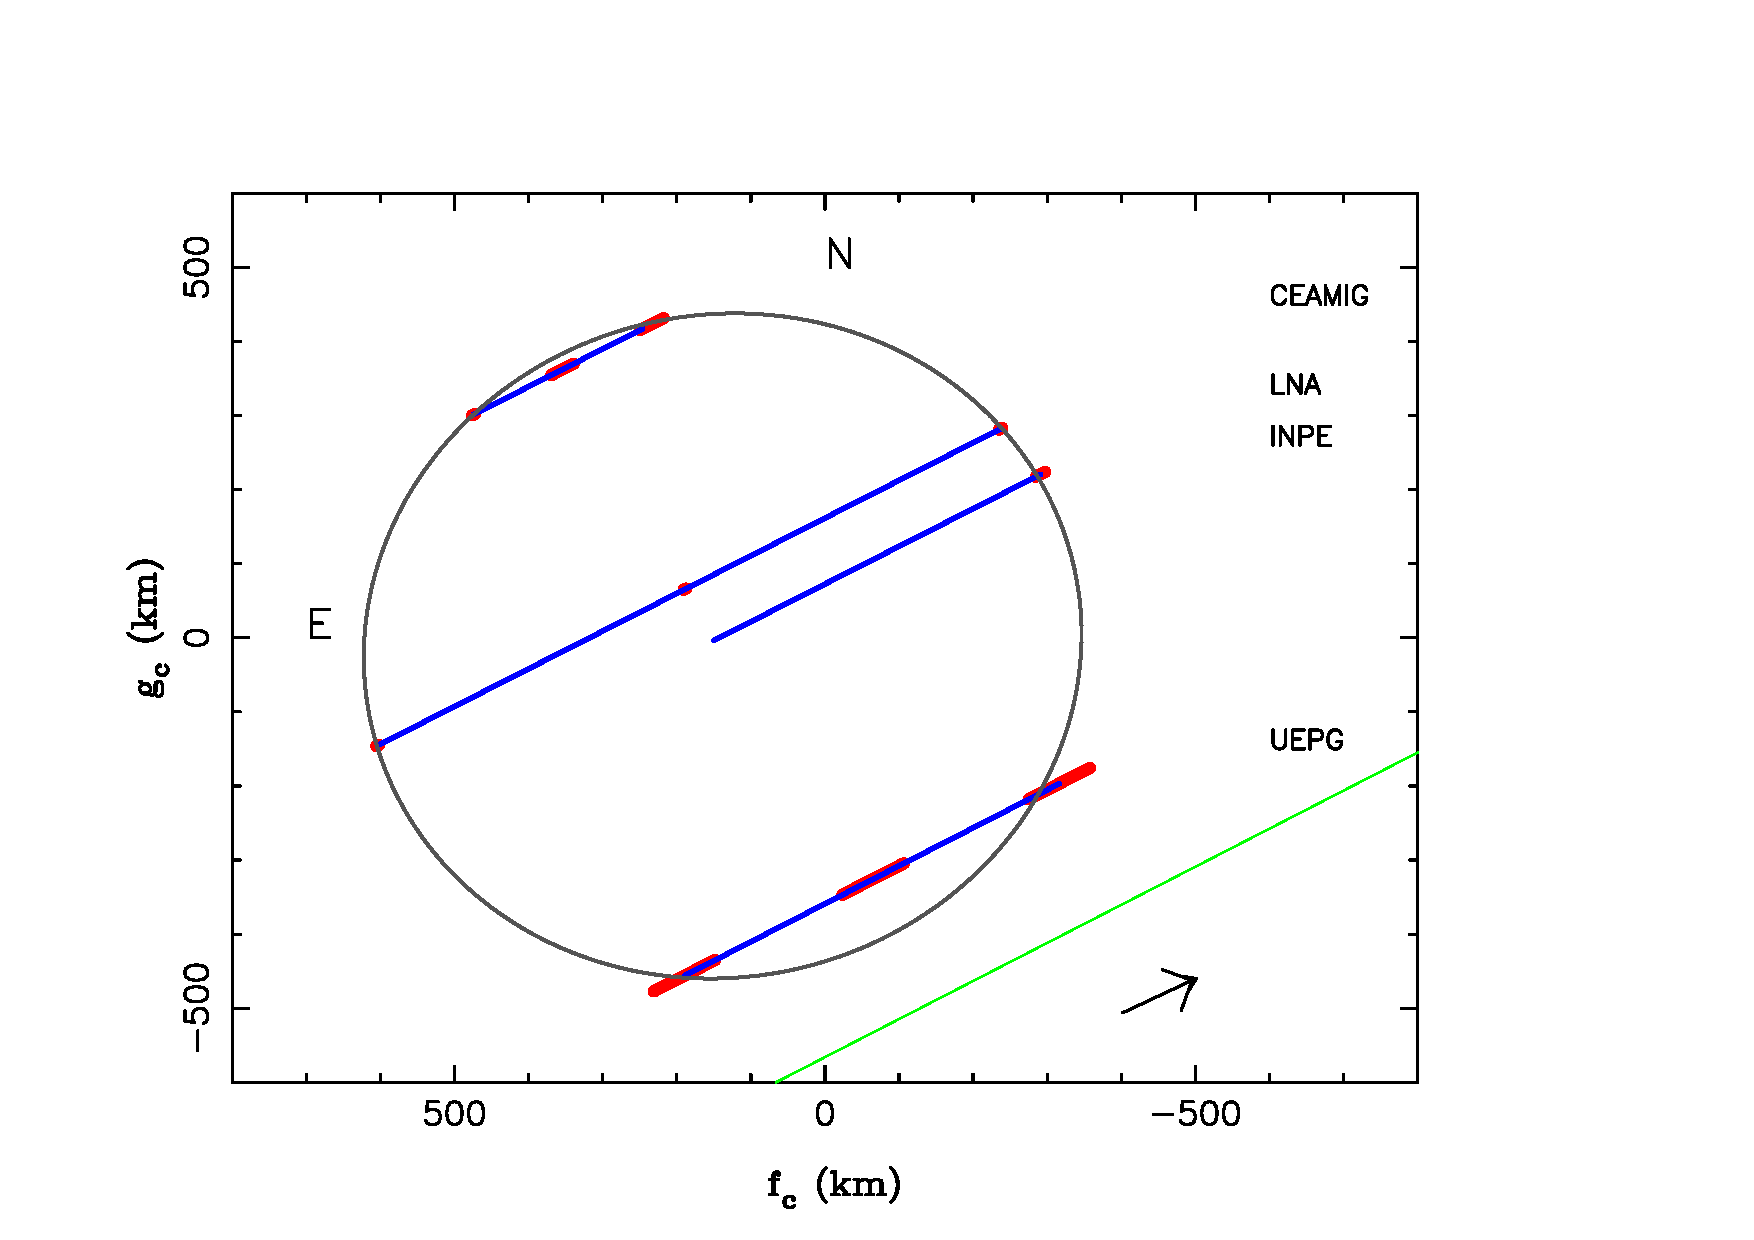
\includegraphics[scale=0.36]{figures/Ceres_2010_body.pdf} 
\caption{The best elliptical fit for the occultation chords for the event of 2010 using the times from Table~\ref{Tab: obs-2010} and the pole-constrained solution. \label{Fig:Ceres-2010-body}}
\end{figure}







\section[]{The 2013 occultation}

\subsection{Observations}\label{Sec: observation-2013}

The event which took place on 25 October 2013 involved the star TYC 865-911-1 (UCAC2 35031360), of magnitude $K = 8.76$. Its ICRF/J2000 position is \citep{Zacharias2004}:
%
\begin{equation}
\left\{ 
  \begin{array}{l l}
    \alpha = 11^{h}57^{m}52^{s}.7641\\
    \delta = +09\degr 07\arcmin 49\arcsec.835.
  \end{array}
\right.
\end{equation}
%
The occultation could only be visible in the United States, before dawn. The shadow would then cross the Atlantic and Africa, but during daylight time.

\begin{figure}
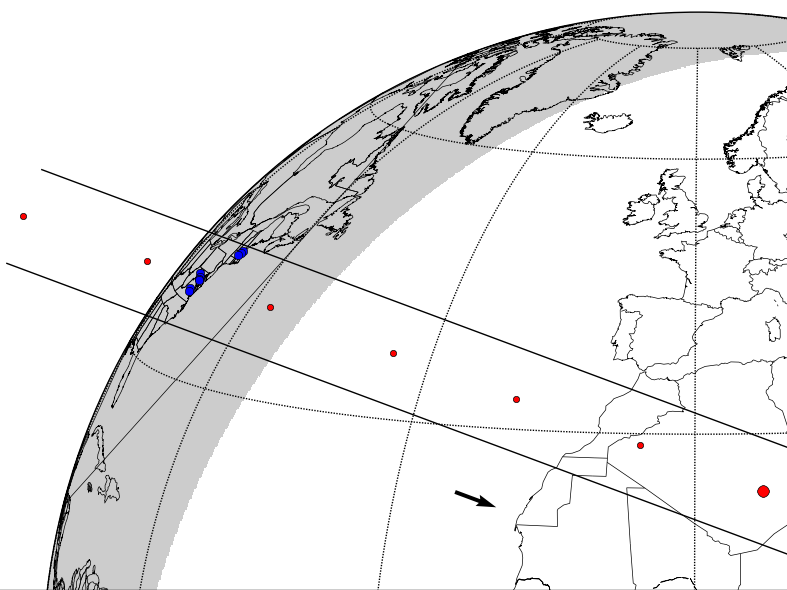
\includegraphics[scale=0.42]{figures/Ceres_2013.png} 
\caption{Post-occultation reconstruction of Ceres' shadow path on Earth for the 2013 October 25 event at the east coast of USA. The big dot is the geocentric closest approach at 09:43:03 UT and the small ones represent the centre of the shadow separated by 30 seconds where the shadow moves from the left to the right. The blue dots are the sites that have observed the event.\label{Fig: Ceres-2013-map}}
\end{figure}

Nine positive chords were obtained by the variety of equipment listed in Table \ref{Tab: obs-2013}. Each station was equipped with a video camera (whose readout time may be considered negligible). This is of particular importance in this event, since Ceres' shadow had the much faster speed of 42.6~km~s$^{-1}$, if compared to the 2010 event. All the observing sites are in the United States, as depicted in Fig.~\ref{Fig: Ceres-2013-map}.

Three different timing synchronization procedures were adopted among the set of observing stations. At Greenbelt and Owings the 1PPS signal of a GPS unit was used to calibrate time stamps which were inserted at each frame of the video. Time extraction is thus straightforward, after taking camera delays into account. On the other hand, at Brookline the clock would be synchronized by an internet server. A lack of connection, however, resulted in spurious times. In fact, comparison between the times obtained at this station and the others suggests that the former have a delay of about 64 s. Therefore, we do not use Brookline's absolute times in the analysis that follows. Finally, at the remaining six stations the videos were recorded by camcorders on digital tapes. The timing method consisted in the comparison of the camcorder internal clock to a 1PPS GPS signal, before and after the recording of the occultation. Absolute timing errors of this procedure are expected to be inferior to 0.1 s.

A remarkable observing circumstance of this event is the low altitude of Ceres with respect to the horizon. Precisely, its altitude at moment of the occultation ranged between $20\degr$ (Hampton) and $15\degr$ (Winchester). Strong scintillation is expected in such a scenario which, combined to short integration times and the low magnitude drop of the event, resulted in rather noisy light curves and thus larger uncertainty in the time of the contacts, as it is shown in the next section.


\begin{table*}
 \centering
 \begin{minipage}{140mm}
  \caption{Circumstances of observation for the observing stations of the 2013 event.\label{Tab: obs-2013}}
  \begin{tabular}{@{}lccccc}
  \hline
     Site & Longitude & Telescope: & Camera  & Result & Observer  \\
          & Latitude  & Aperture  & Cycle time & Ingress & \\          
          & Height    & f-ratio    &    S/N    & Egress    & \\          
\hline
 Hampton & 70$\degr$48'59.7'' W & 12 cm & PC164C-EX2 & Positive & T. Blank \\
  &42$\degr$53'52.8'' N & f/5 & 0.033 s     & 09:40:46.9 $\pm$ 0.1 &   \\
            & 7 m       &  &     & 09:40:57.26  $\pm$ 0.08 &   \\
 & & & & & \\
 Topsfield & 70$\degr$55'16.6'' W & 12 cm & PC164C-EX2 & Positive & T. Blank \\
  &42$\degr$37'55.9'' N & f/5      & 0.033 s   & 09:40:45.4 $\pm$ 0.1 &   \\
            & 45 m      &  &     & 09:40:58.0  $\pm$ 0.1 &   \\
 & & & & & \\
 Brookline & 71$\degr$08'14.5'' W & 64 cm & Infinity2-1R & Positive & N. Weber \\
  &42$\degr$18'27.4'' N & f/9.6 & 0.015 s     & Duration only &  R. Dantowitz  \\
            & 109 m     &       &     & (14.93 $\pm$ 0.01) s &   \\
 & & & & & \\
 Winchester & 78$\degr$14'39.6'' W & 36 cm & PC164C & Positive & J. Brooks \\
  &39$\degr$16'21.5'' N & f/5 & 0.033 s    & 09:40:33.26 $\pm$ 0.08 &   \\
            & 211 m     &  &     & 09:40:55.86  $\pm$ 0.09 &   \\
 & & & & & \\
 Greenbelt & 76$\degr$52'09.4'' W & 12 cm & PC164C-EX2 & Positive & J. Dunham \\
  &38$\degr$59'12.1'' N & f/2.5 & 0.033 s    & 09:40:33.6 $\pm$ 0.1 & D. Dunham  \\
            & 52 m      &   &     & 09:40:56.4  $\pm$ 0.1 &   \\
 & & & & & \\
 Alexandria & 77$\degr$02'28.3'' W & 7 cm & Watec120N & Positive & P. Maley \\
  &38$\degr$49'19.1'' N & f/10 &  0.067 s   & 09:40:33.3 $\pm$ 0.1 &   \\
            & 8 m       &   &     & 09:40:56.1  $\pm$ 0.1 &   \\
 & & & & & \\
 Owings & 76$\degr$38'06.3'' W & 25 cm & PC164C  & Positive & C. Ellington \\
  &38$\degr$41'26.5'' N & f/3.3 &  0.033 s & 09:40:34.27 $\pm$ 0.05 &   \\
            & 38 m                &       &     & 09:40:56.0  $\pm$ 0.2 &   \\
 & & & & & \\
 Mechanicsville & 77$\degr$23'06.7'' W & 12 cm & PC164C-EX2 & Positive & D. Dunham \\
  &37$\degr$41'26.1'' N & f/2.5 & 0.033 s    & 09:40:33.0 $\pm$ 0.1 &   \\
            & 60 m      &   &     & 09:40:54.8  $\pm$ 0.1 &   \\
 & & & & & \\
 Varina & 77$\degr$19'49.3'' W & 12 cm & PC164C-EX2 & Positive & D. Dunham \\
  &37$\degr$25'58.6'' N & f/2.5 &  0.033 s   & 09:40:32.4 $\pm$ 0.3 &   \\
            & 19 m      &   &     & 09:40:53.1  $\pm$ 0.2 &   \\

\hline
\end{tabular}
\end{minipage}
\end{table*}

\subsection{Light curves and timing}

All videos were converted to FITS images and the photometry of the target was obtained via the PRAIA \citep{2011gfun.conf...85A}. The light curves were normalized to the flux of a reference star when such was available on the field.

To reduce the noise, the data were binned by groups of five images -- with the exception of  Greenbelt, which was averaged in sets of ten. This procedure enlarges the effective integration times reported in Table~3 by a factor of 5 (or 10). As in the 2010 event, an additional normalization by a polynomial curve was applied.

The start and end times of the occultation were obtained by the same procedure explained in Section~2.2. The Fresnel scale of 0.4~km for this event was calculated using Ceres' geocentric distance $D = 3.28 \text{ au} = 4.91 \times 10^{8}$~km, for a typical wavelength of $\lambda = 0.65$~$\micron$. Considering the apparent magnitudes of the star, $B = 10.47$, $V=9.97$, and $K=8.76$ \citep{Hog2000}, we estimate its diameter projected at Ceres' distance as 0.16~km. Thence, since the typical effective integration time used (0.17~s) translates to about 7 km in the celestial plane, theoretical occultation light curves are largely dominated by the integration times, as for the 2010 event.

The best-fittings to the occultation light curves are shown in Fig.~\ref{Fig: Ceres-2013-curves}, and the derived occultation times are listed in Table~\ref{Tab: obs-2013}.

\begin{figure}
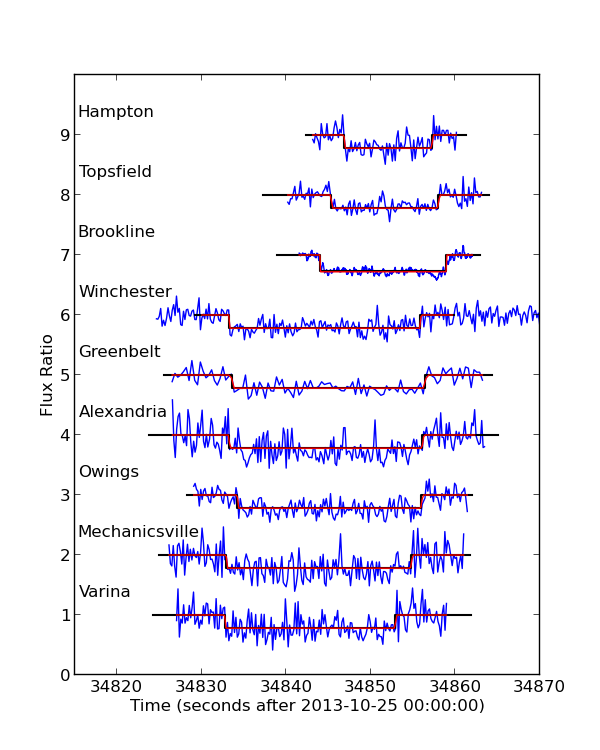
\includegraphics[scale=0.58]{figures/Ceres_2013_fluxratio} 
\caption{The nine occultation light curves normalized and vertically shifted by a factor of 1.0 for better viewing. The solid black lines are the best fit of the square-well model to the data. The red lines are the square-well model convoluted with the Fresnel diffraction, the star diameter, and the applied exposure time. The mid-times of the occultations do not coincide due to the propagation delays of the shadow due to the distinct longitude of the sites. The light curve of Brookline is shifted by -64 s as explained in the text. \label{Fig: Ceres-2013-curves}}
\end{figure}






\subsection{Limb fitting solutions}

Elliptic limb profiles were adjusted to the eight\footnote{Brookline's chord was not used for limb fitting since it actually measured duration instead of absolute times.} chords by the same procedure described in Section~\ref{Sec: limbfittingmethod}. This yielded $\chi^2_{r,min} = 13$, suggesting that an elliptic model is not satisfactory to the data. Indeed, a quick glance at a plot of the observed chords --such as in Fig.~\ref{Fig: Ceres-2013-body}-- shows that the Varina chord seems to be somewhat advanced with respect to the others. Taking into account that in this station time stamps were not inserted on the video frames, it is always possible to attribute this advance to an eventual problem on the correspondence between camcorder's and GPS' times. This could be caused, for example, if the camcorder delayed to start the recording and, since this was an unattended pre-pointed station, this fact would not be noticed by the analysis of the video itself.

The immersion recorded at Owings also seems to be shifted (delayed) with respect to the nearby chords --see Fig.~\ref{Fig: Ceres-2013-body}. This chord, actually, has roughly the same length of Mechanicsville's, despite the fact that they are separated by circa 100~km. Differently from Varina, though, this station had time stamps inserted in each frame of the video, which makes it more unlike to justify an eventual timing issue. Another possible explanation for the times of this chord is the determination of the events in the light curve analysis, which could have been affected by noise. Finally, the delay during the ingress could be caused by a relief feature in Ceres; we shall soon return to this hypothesis.

%In addition to a time basis problem, other possible explanations to the times of this chord are the determination of the events in the light curve analysis, due to noise; and finally that the delay during the ingress could be caused by a relief feature in Ceres. 

In a second limb fitting, thus, we did not consider Brookline, Varina and Owings chords. The adjust of the five parameters which define an ellipse to the 12 contacts then resulted in $\chi^2_{r,min} = 1.27$, indicating that the fitting is in good agreement with the observed data within the error bars. This is the solution depicted in Fig.~\ref{Fig: Ceres-2013-body}, where we see that the chord length measured in Brookline is compatible to the model. The associated physical parameters are presented in Table~2 as the nominal solution.

For this event the polar aspect angle is $\zeta = 90.7\degr$, which makes true oblateness be equal to the apparent one, within the error bars.

It is worth noting that the position angle of this nominal solution is better constrained than the respective of the 2010 occultation. Actually, the uncertainty of the former is of $5\degr$ in contrast to $10\degr$ of the latter. This suggests that the pole-constrained solution obtained via the position of Ceres' pole (\ref{Pole}) would not be significantly different of the nominal one.

This assumption is confirmed when we carry out the limb fitting with the constraint $P = (25 \pm 3)\degr$ --the position angle at the moment of the occultation which follows from (\ref{Pole}). The physical parameters related to this pole-constrained solution are presented in the last column of Table~2, and are essentially the same of the nominal solution.

We close this section returning to the hypothesis that the delay observed in the immersion at Owings could be associated to a limb topography feature. The recorded contact would then correspond to a negative elevation of $31 \pm 4$ km with respect to the best-fitting ellipse. Theoretical models, however, predict that relief in Ceres should be no higher than about 10--20 km \citep{Johnson1973}, while published observational data sets the bound of 18 km \citep{Carry2008}. More recently, images by the probe \textit{Dawn} also reveal an even smoother surface. The association of Owings first contact to a relief must, therefore, be ruled out.

\begin{figure}
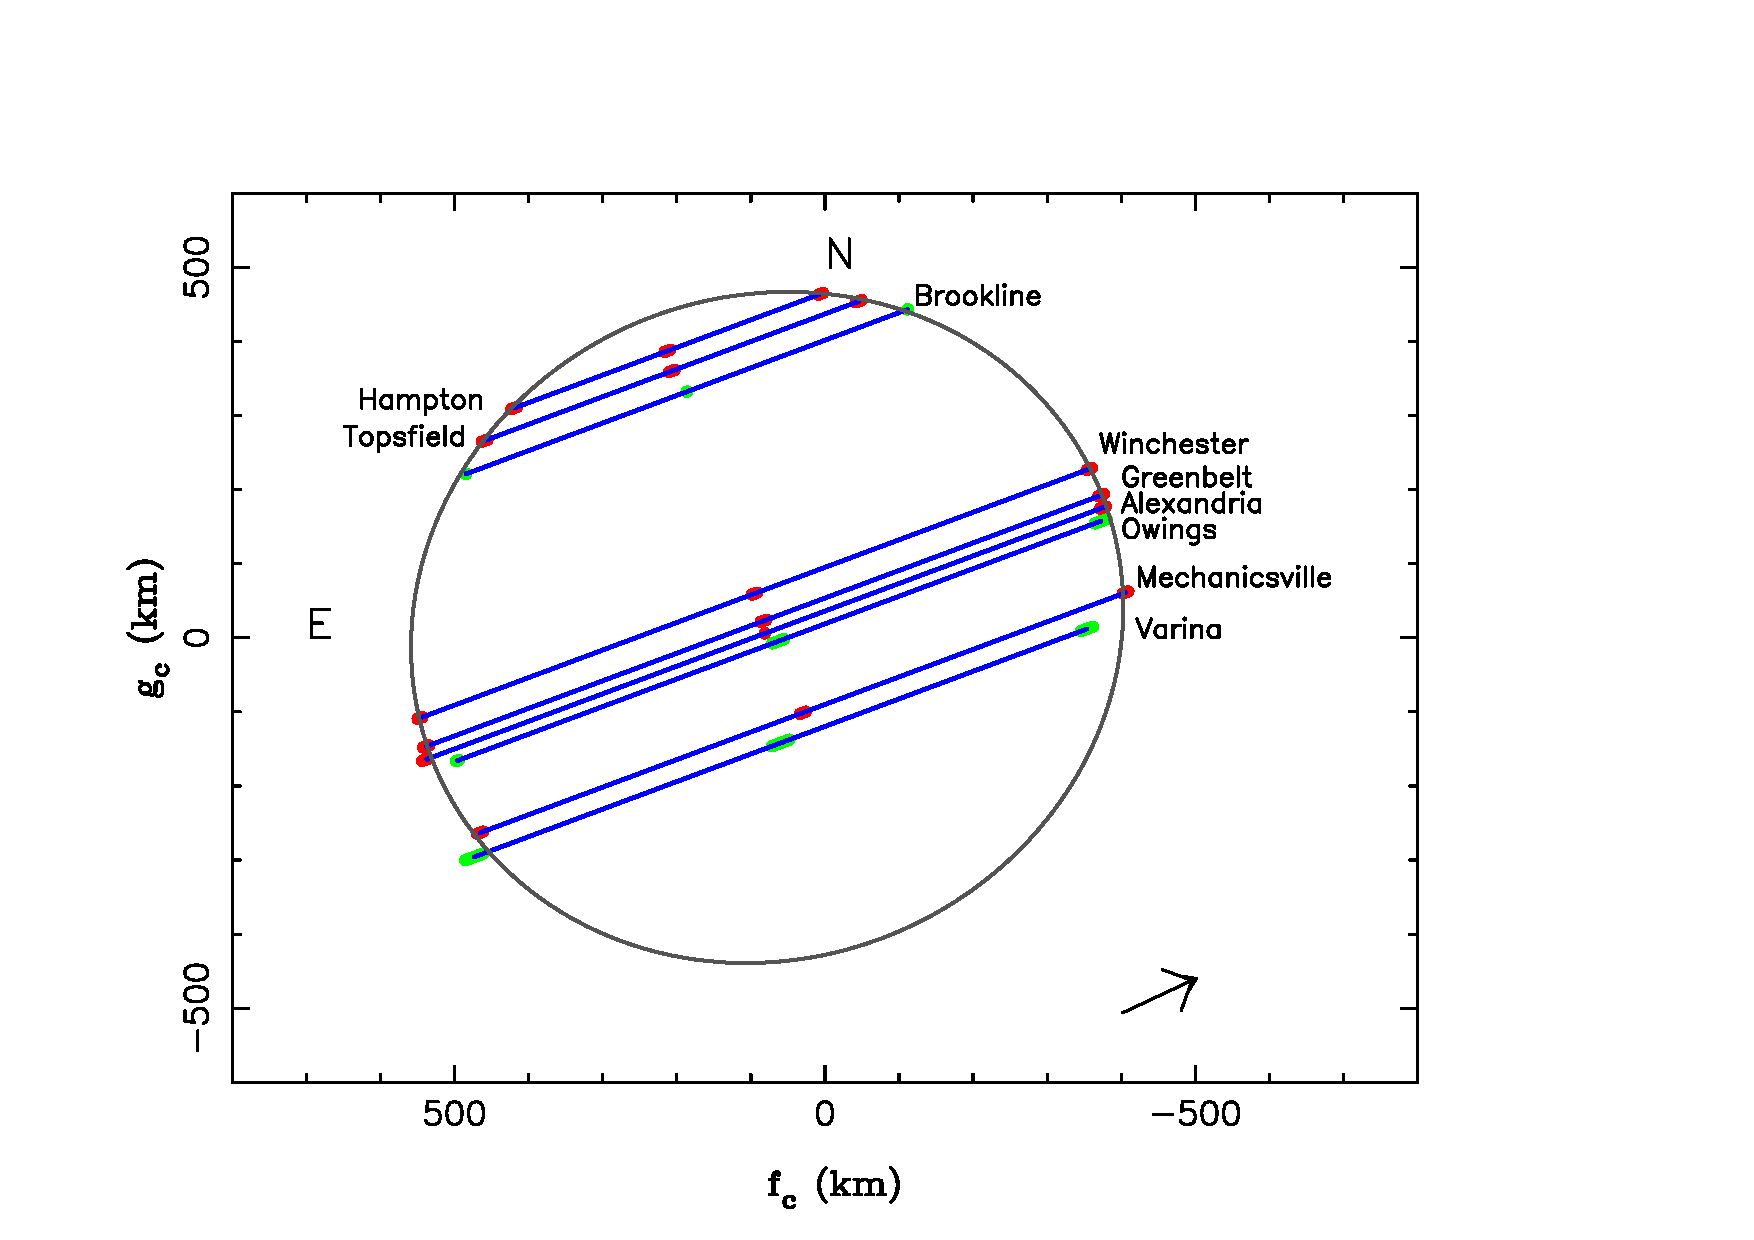
\includegraphics[scale=0.36]{figures/Ceres_2013_body.pdf}
\caption{The best elliptical fit for the occultation chords for the event of 2013 using timing from Table \ref{Tab: obs-2013} and the nominal solution. The chord of Brookline if shifted by -64s as explained in the text\label{Fig: Ceres-2013-body}}
\end{figure}




\section[]{Discussion}

A quick glance at Table~2 shows there is an overall agreement between the physical parameters derived from both occultations, specially in the equatorial diameter. The differences of the solutions occur basically on the size of their error bars, and can be justified by the particularities of each set of data.

The 2010 event, for example, had only seven contacts; none the less, they were well distributed over Ceres' disc (see Fig.~\ref{Fig:Ceres-2010-body}) acting as a constraint to is shape. On the other hand, the 2013 event had five more contacts, but they were concentrated in certain regions of the body. In particular, the absence of chords closer to Ceres' southern limb made its oblateness be worse determined here than in the 2010 event.

However, even our best measurement for the oblateness, $\epsilon=0.08 \pm 0.03$, has still a big uncertainty with regard to other figures published in the literature, as Table~4 shows. A larger number of uniformly spaced chords would be necessary to offer a best constraint to the oblateness.

The few chords of the 2010 occultation could themselves only constraint the position angle of the object to a $20\degr$ interval. This range was reduced by a factor of two in the 2013 event, approaching --and verifying-- the result predicted by the work of \cite{Drummond2014}. As it was shown, using the coordinates of Ceres' polar axis to limit the position angle was not an efficient procedure in the case of this occultation, in the sense that the aforementioned limitation had not correspond to a stronger constraint on the other parameters.

On the other hand, constraining the position angle on the 2010 occultation was proved to reduce the error bars of the other parameters (disregarding oblateness). Moreover, this procedure resulted in an excellent agreement between the equatorial radius figures of both events.

The 2013 occultation, therefore, offers not only an independent verification of the figures resulted from the 2010 event, but also validates the procedure carried out there --and which led to the best-constrained parameters in this work.

Comparison of Ceres' equatorial diameter as measured by different techniques is carried out in Table~4. We note an overall agreement between our result to those obtained via direct imaging by the Hubble Space Telescope (HST) \citep{Thomas2005}, the Keck Observatory and the ESO VLT \citep{Drummond2014}. The smaller figure reported by \cite{Carry2008} may be justified by the fact that in this study the effects of limb-darking were not taken into account, as pointed out by \cite{Drummond2014}.

As mentioned in the Introduction, the 1984 event \citep{Millis1987} is the only occultation data to which we can compare our result; and it is interesting to notice that the diameters measured in each case do not agree, being our result larger than the other. It is difficult to state with sure the reasons for this divergence since we had no access to the original 1987 data or reduction methodology. We note, however, that in this occultation a variation of 0.5 s in the contact times correspond to almost 7~km on Ceres' limb. Therefore, in order to properly compare their result to ours it would be necessary to reduce their light curves with the same methodology used in the present work.



\begin{table*}
 \centering
 \begin{minipage}{140mm}
  \caption{Ceres' equatorial diameter and oblateness}
  \begin{tabular}{@{}llcc}
  \hline
     Eq. diameter (km) & Oblateness & Method & Ref. \\
\hline
$972 \pm 6$  & $0.08  \pm 0.03$  & Occultation & 1\\
$967 \pm 10$ & $0.078 \pm 0.015$ & Keck+VTL    & 2 \\
$959 \pm 5$  & $0.074 \pm 0.007$ & Keck        & 3\\
$975 \pm 4$  & $0.068 \pm 0.005$ & HST         & 4\\
$959 \pm 5$  & $0.05  \pm 0.01$  & Occultation & 5\\
\hline
\end{tabular}
\textbf{References.} 1: Present work. 2: \cite{Drummond2014}. 3: \cite{Carry2008}. 4: \cite{Thomas2005}. 5: \cite{Millis1987}.
\end{minipage}
\end{table*}



\section*{Acknowledgements}

Agradecimentos


\begin{thebibliography}{99}

\bibitem[\protect\citeauthoryear{Assafin et al}{2011}] {2011gfun.conf...85A} Assafin M. et al., 2011, Gaia follow-up network for the solar system objects : Gaia FUN-SSO workshop proceedings, held at IMCCE -Paris Observatory, France, November 29 - December 1, 2010. ISBN 2-910015-63-7

%@INPROCEEDINGS{2011gfun.conf...85A,
%   author = {{Assafin}, M. and {Vieira Martins}, R. and {Camargo}, J.~I.~B. and 
%	{Andrei}, A.~H. and {Da Silva Neto}, D.~N. and {Braga-Ribas}, F.
%	},
%    title = "{PRAIA - Platform for Reduction of Astronomical Images Automatically}",
%booktitle = {Gaia follow-up network for the solar system objects : Gaia FUN-SSO workshop proceedings, held at IMCCE -Paris Observatory, France, November 29 - December 1, 2010. ISBN 2-910015-63-7},
%     year = 2011,
%   editor = {{Tanga}, P. and {Thuillot}, W.},
%    month = jun,
%    pages = {85-88},
%   adsurl = {http://adsabs.harvard.edu/abs/2011gfun.conf...85A},
%  adsnote = {Provided by the SAO/NASA Astrophysics Data System}
%}

\bibitem[\protect\citeauthoryear{Braga-Ribas et al.}{2013}]{BragaRibas2013} Braga-Ribas F. et al., 2013,
ApJ, 773, 26

\bibitem[\protect\citeauthoryear{Braga-Ribas et al.}{2014}]{BragaRibas2014} Braga-Ribas F. et al., 2014,
Nature, 508, 72

\bibitem[\protect\citeauthoryear{Drummond et al.}{2014}]{Drummond2014} Drummond J.D. et al., 2014,
Icarus, 236, 28

\bibitem[\protect\citeauthoryear{Carry et al.}{2008}] {Carry2008} Carry B. et al., 2008,
A\&A, 478, 235

\bibitem[\protect\citeauthoryear{Hog et al.}{2000}] {Hog2000} Hog E. et al., 2000,
A\&A, 355, L27

\bibitem[\protect\citeauthoryear{Johnson \& McGetchin}{1973}] {Johnson1973} Johnson T.V., McGetchin T.R., 1973,
Icarus, 18, 612

\bibitem[\protect\citeauthoryear{K\"{u}ppers et al.}{2014}]{Kuppers2014} K\"{u}ppers M. et al., 2014,
Nature, 505, 525

\bibitem[\protect\citeauthoryear{Millis et al.}{1987}]{Millis1987} Millis R.L. et al., 1987,
Icarus, 72, 507

%\bibitem[\protect\citeauthoryear{Ortiz et al.}{2012}]{Ortiz2012} Ortiz J.L. et al., 2012,
%Nature, 491, 566

\bibitem[\protect\citeauthoryear{Sicardy et al.}{2011}]{Sicardy2011} Sicardy B. et al., 2011,
Nature, 478, 493

\bibitem[\protect\citeauthoryear{Thomas et al.}{2011}]{Thomas2005} Thomas P.C. et al., 2005,
Nature, 437, 224

\bibitem[\protect\citeauthoryear{Widemann et al.}{2009}] {Widemann2009} Widemann T. et al., 2009,
Icarus, 199, 458

\bibitem[\protect\citeauthoryear{van Belle}{1999}] {vanBelle1999} van Belle G.T., 1999,
PASP, 111, 1515

\bibitem[\protect\citeauthoryear{Zacharias et al.}{2004}]{Zacharias2004} Zacharias N. et al., 2004,
AJ, 127, 3043
















%Artigos do exemplo

%\bibitem[\protect\citeauthoryear{Dawson}{1979}]{b4} Dawson D.W., 1979,
%ApJS, 41, 97
%\bibitem[\protect\citeauthoryear{Gerhz}{1972}]{b5} Gerhz R.D., 1972, ApJ,
%178, 715
%\bibitem[\protect\citeauthoryear{Gerhz \& Ney}{1972}]{b6} Gerhz R.D., Ney
%E.P., 1972, PASP, 84, 768
%\bibitem[\protect\citeauthoryear{Gerhz \& Woolf}{1970}]{b7} Gerhz R.D., Woolf N.J.,
%1970, ApJ, 161, L213
%\bibitem[\protect\citeauthoryear{Gilman}{1972}]{b8} Gilman R.C., 1972, ApJ, 178, 423
%\bibitem[\protect\citeauthoryear{Goldsmith et al.}{1987}]{b9} Goldsmith M.J., Evans A.,
%Albinson J.S., Bode M.F., 1987, MNRAS, 227, 143
%\bibitem[\protect\citeauthoryear{Hacking et al.}{1985}]{b10} Hacking P. et al., 1985,
%PASP, 97, 616
%\bibitem[\protect\citeauthoryear{Harvey, Thronson \& Gatley}{Harvey et al.}{1979}]{b11}
%Harvey P.M., Thronson H.A., Gatley I., 1979, ApJ, 231, 115
%\bibitem[\protect\citeauthoryear{Jura}{1986}]{b12} Jura M., 1986, ApJ, 309, 732
%\bibitem[\protect\citeauthoryear{Kukarkin et al.}{1969}]{b13} Kukarkin B.V. et al.,
%1969, General Catalogue of Variable Stars. Moscow
%\bibitem[\protect\citeauthoryear{Lloyd Evans}{1974}]{b14} Lloyd Evans T., 1974, MNRAS,
%167, 17{\sc p}
%\bibitem[\protect\citeauthoryear{Lloyd Evans}{1985}]{b15} Lloyd Evans T., 1985, MNRAS,
%217, 493
%\bibitem[\protect\citeauthoryear{Low et al.}{1984}]{b16} Low F.J. et al., 1984, ApJ,
%278, L19
%\bibitem[\protect\citeauthoryear{McLaughlin}{1932}]{b17} McLaughlin D.B., 1932, Publ. Univ.
%Obs. Mich., 4, 135
%\bibitem[\protect\citeauthoryear{O'Connell}{1961}]{b18} O'Connell J.K., 1961, Specola
%Vaticana Ric. Astron., 6, 341
%\bibitem[\protect\citeauthoryear{Olnon \& Raimond}{1986}]{b19} Olnon F.M., Raimond E., 1986,
%A\&AS, 65, 607
%\bibitem[\protect\citeauthoryear{Preston et al.}{1963}]{b20} Preston G.W., Krzeminski W., Smak J.,
%Williams J.A., 1963, ApJ, 137, 401
%\bibitem[\protect\citeauthoryear{Rowan-Robinson \& Harris}{1983a}]{b21} Rowan-Robinson M., Harris
%S., 1983a, MNRAS, 202, 767
%\bibitem[\protect\citeauthoryear{Rowan-Robinson \& Harris}{1983b}]{b22} Rowan-Robinson M., Harris
%S., 1983b, MNRAS, 202, 797
%\bibitem[\protect\citeauthoryear{van der Veen \& Habing}{1988}]{b23} van der Veen W.E.C.J., Habing
%H.J., 1988, A\&A, 194, 125
%\bibitem[\protect\citeauthoryear{Willems \& de Jong}{1988}]{b24} Willems F.J., de Jong T., 1988,
%A\&A, 196, 173
%\bibitem[\protect\citeauthoryear{Zuckerman \& Dyck}{1986}]{b25} Zuckerman B., Dyck H.M., 1986, ApJ,
%311, 345
\end{thebibliography}



%\bsp

\label{lastpage}

\end{document}